\documentclass[UTF8, 12pt]{ctexart}

\usepackage{amsmath}

\usepackage{geometry}
\geometry{a4paper, scale = 0.9} % a4纸, 版心占页面长度的比例为0.9

\usepackage{enumitem} % itemize, 列表

\usepackage{graphicx}

\begin{document}

	\noindent
	特点 :
	\begin{itemize}[leftmargin = 4em]
		\item 除了放大区, 饱和区, 截止区, 还有过电流区($ I_{C} > I_{CM} $), 过电压区($ U_{CE} > U_{(BR)CEO} $), 过损耗区($ P_{CM} = I_{C}*U_{CE} $)
		\item 非线性失真小
		\item 效率高, $ \eta = \frac{\text{负载得到的功率}}{\text{电源提供的功率}} $
	\end{itemize}

	分类 : 甲类(一个周期内有电流流过晶体管), 乙类(只有半个周期导通), 甲乙类(大于半个小于一个), 丙类(小于半个)

	~

	\noindent
	甲类功率放大器 :

	电路图 :

	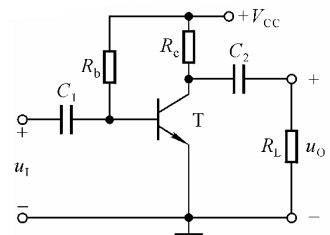
\includegraphics[scale = 0.4]{04/甲类功率放大器电路图.png}

	分析 :
	\begin{itemize}[leftmargin = 4em]
		\item 输出功率 : $ P_{o} = I_{o}U_{o} = \frac{1}{2}I_{om}U_{om} $
		\item 最大幅值 : $ U_{cem} = \frac{1}{2}(V_{CC}-U_{CES}), I_{cm}=I_{CQ}, P_{o} = \frac{1}{4}I_{CQ}V_{CC} $ (忽略 $ U_{CES} $)
		\item 电压源功率 : $ P_{v} = \frac{1}{2\pi} \int_{0}^{2\pi}V_{CC}i_{c}\mathrm{d}\omega t = \frac{1}{2\pi} \int_{0}^{2\pi}V_{CC}(I_{CQ}+I_{Cm}s\sin\omega t)\mathrm{d}\omega t = V_{CC}I_{CQ} $
		\item 最高效率 : $ \eta = 25\% $
	\end{itemize}

	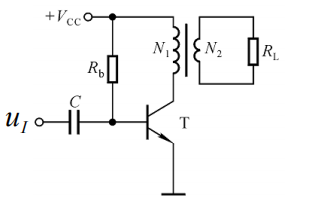
\includegraphics[scale = 0.4]{04/变压器耦合功率放大器电路图.png}

	分析 :
	\begin{itemize}[leftmargin = 4em]
		\item 直流负载线是垂直于x轴的
		\item 输出功率 $ P_{o} = \frac{1}{2}I_{om}U_{om} $, 最大输出功率 $ P_{om} = \frac{1}{2}I_{CQ}V_{CC} $, 最高效率 $ \eta = 50\% $
	\end{itemize}

	~

	\noindent
	乙类功率放大器 :

	电路图 :

	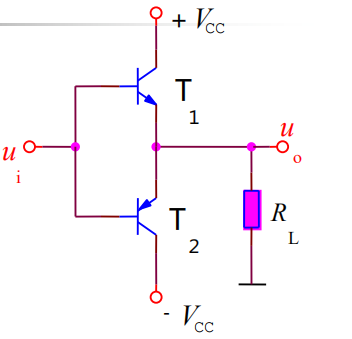
\includegraphics[scale = 0.4]{04/乙类功率放大电路电路图.png}

	分析 :
	\begin{itemize}[leftmargin = 4em]
		\item 静态时, 两管均截止; 动态时, 两管交替工作, 在负载上得到完整波形
		\item 输出功率 : $ P_{o} = \frac{1}{2}\frac{U_{om}^{2}}{R_{L}}, P_{om} = \frac{1}{2}\frac{U_{om}^{2}}{R_{L}} \approx \frac{1}{2}\frac{V_{CC}}{R_{L}} $
		\item 电源功率 : $ P_{v} = 2*\frac{1}{2\pi} \int_{0}^{2\pi}|V_{CC}i_{C1}|\mathrm{d}\omega t = \frac{1}{\pi}V_{CC}I_{om}\sin\omega t\mathrm{d}\omega t = \frac{2}{\pi}\frac{V_{CC}U_{om}}{R_{L}} $
		\item 三极管管耗最大在 $ U_{om} = \frac{2}{\pi}V_{CC} $ 处
		\item 最高效率 : $ \eta = \frac{\pi}{4} $
		\item 交越失真 : 输入信号很小的时候, 达不到三极管的开启电压, 在正负半周交替过零处出现非线性失真
	\end{itemize}

	单电源OTL互补功率放大电路

	电路图 :

	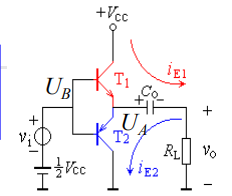
\includegraphics[scale = 0.4]{04/单电源OTL互补功率放大电路.png}

	分析 :
	\begin{itemize}[leftmargin = 4em]
		\item 和双电源的乙类放大器比, 只需把公式里的 $ V_{CC} $ 换成 $ V_{CC}/2 $ 即可
		\item 两个三极管正半周负半周轮流放电
 	\end{itemize}

	~

	\noindent
	甲乙类功率放大器 :

	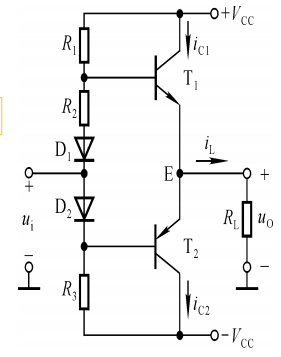
\includegraphics[scale = 0.4]{04/甲乙类功率放大器电路图.png}

	分析 :
	\begin{itemize}[leftmargin = 4em]
		\item 静态 : $ U_{B1B2} = U_{R2}+U_{D1}+U_{D2} $, 两管微弱导通, 每管导通时间大于半个周期
	\end{itemize}

	复合管 : $ T_{1} $ 的c端连接 $ T_{2} $ 的c端, $ T_{1} $ 的e端连接 $ T_{2} $ 的b端, $ T_{1} $ 的b, $ T_{2} $ 的ce作为复合管的bce, $ \beta = \beta_{1}\beta_{2} $, 管子类型和$ T_{1} $ 相同

	带复合管的OCL互补输出功放电路 :

	电路图 :

	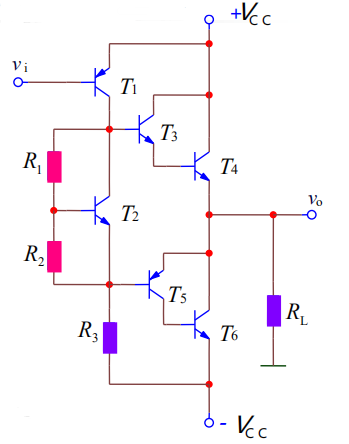
\includegraphics[scale = 0.4]{04/带复合管的OCL互补输出功放电路电路图.png}


\end{document}